\section{Implementation}

In this section, we describe the implementation of our fault tolerance
strategies as an extension to \themis. Section~\ref{sec:themis} provides a
brief overview of \themis' architecture, and Section~\ref{sec:recovery}
describes the implementation of our write and read recovery strategies in the
context of that architecture. In Section~\ref{sec:multi-tenancy}, we describe
extensions to \themis to support multi-tenancy. Section~\ref{sec:control_plane}
describes the way that jobs are dispatched.
Section~\ref{sec:input_file_gathering} describes how files are assigned to
nodes, and explores the practical concern of achieving high bandwidth from
distributed storage. Section~\ref{sec:fault_response} describes how failures
are detected and how nodes respond to failure during a job.

\subsection{Themis: I/O-Efficient MapReduce}
\label{sec:themis}

In this section, we present a brief recap of the design of \themis, our highly
I/O-efficient MapReduce system. A more detailed description and evaluation of
\themis is presented in Chapter~\ref{chapter:themis}.  We opted to implement
our fault tolerance scheme in \themis rather than Hadoop because \themis lacked
a proportional fault tolerance mechanism prior to this work, whereas the
task-level fault tolerance scheme used by Hadoop is a tightly-integrated part
of its design.

\begin{figure}
  \centering
  \begin{subfigure}[t]{\columnwidth}
  \centering
  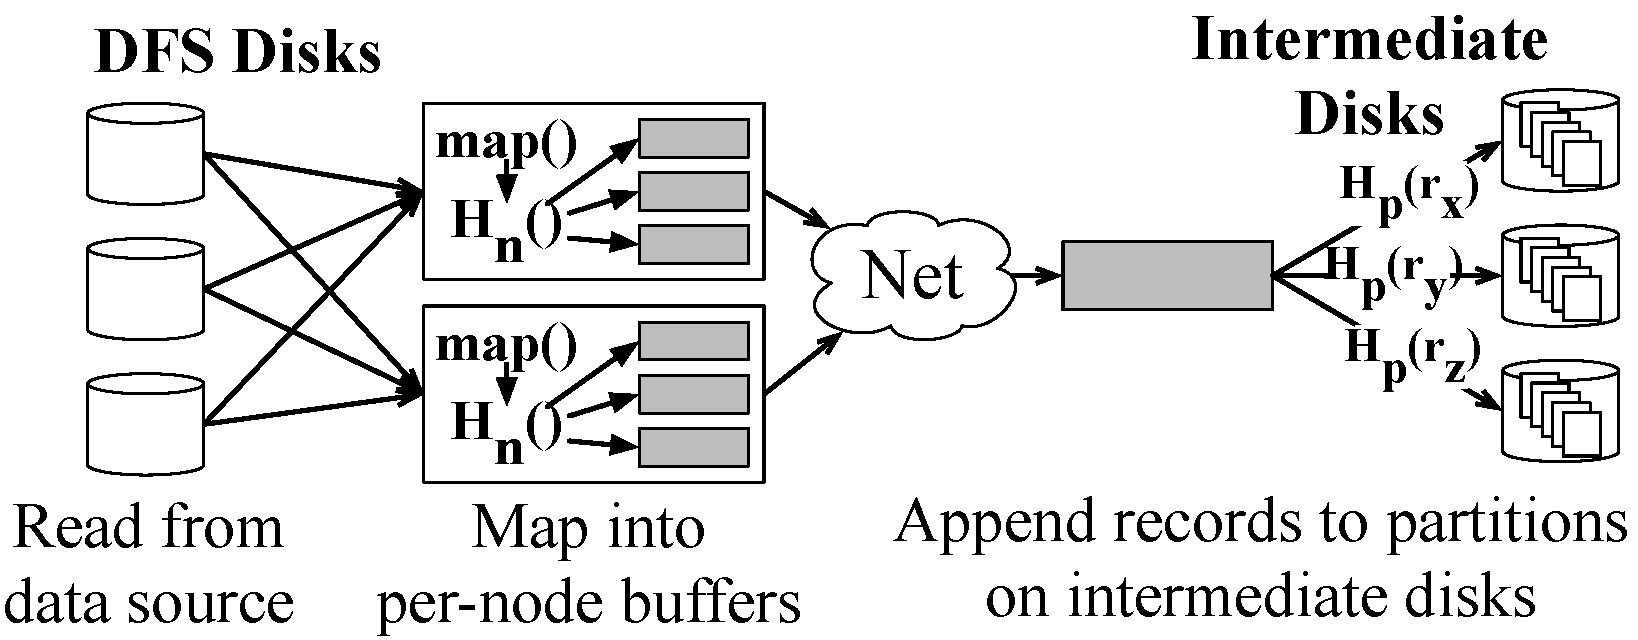
\includegraphics[width=\columnwidth]{fault_tolerance/figures/detailed_phase_one.pdf}
  \caption{\label{fig:phase_one} Phase One}
  \end{subfigure}\vspace{1em}
  \begin{subfigure}[t]{\columnwidth}
  \centering
  
\includegraphics[width=\columnwidth]{fault_tolerance/figures/phase_two.pdf}
  \caption{\label{fig:phase_two} Phase Two}
  \end{subfigure}

  \caption{\label{fig:themis_phases} A diagrammatic overview of \themis' phases.}
\end{figure}

Nodes in a \themis cluster each have a collection of \emph{intermediate disks}
that store volatile intermediate data and a disjoint collection of \emph{DFS
  disks} that store input and output data, and are typically under the control
of a distributed file system like HDFS.

\themis runs a MapReduce job in two main \emph{phases}, called \emph{phase one}
and \emph{phase two}.  In phase one, input records are read in parallel from
the cluster's DFS disks. \themis applies the \map function to each record,
producing a collection of \emph{intermediate records} that are written to
intermediate partitions spread across the cluster's intermediate disks. Each
intermediate partition holds all records with a certain set of keys. The
mapping from keys to intermediate partitions is determined by a \emph{partition
  function}. Phase one is roughly analogous to Hadoop's map and shuffle phases.

At the end of phase one, all intermediate records have been generated,
partitioned and stored across the cluster's intermediate disks. A diagrammatic
overview of phase one is given in Figure~\ref{fig:phase_one}.

In phase two, each intermediate partition is read from the cluster's
intermediate disks completely into memory. Once in memory, it is sorted in-core
by key, and the \reduce function is applied to each group of records in the
partition with the same key. This produces a collection of \emph{output
  records} that are written to files on the DFS disks. Phase two is roughly
equivalent to Hadoop's sort and reduce phases. A diagrammatic overview of phase
two is given in Figure~\ref{fig:phase_two}.

Note that phase one requires all-to-all communication among cluster nodes, but
that phase two can be executed on each node independently.

\subsubsection{Partitioning}

In order for phase two to be processed efficiently, partitions should be small
enough for several of them to be processed in memory
simultaneously. Additionally, they should be as uniformly-sized as possible to
prevent stragglers. The partition function is responsible for ensuring both
these properties. The user can provide their own partition function, or it can
be derived at runtime through an optional sampling phase called \emph{phase
  zero}. Phase zero requires a fairly small sample to produce a good partition
function, and typically takes under a minute to run.


\subsection{Recovery Mechanism}
\label{sec:recovery}

As described in Section~\ref{fault_tolerance:sec:design}, recovering from a
failure consists of two central actions: write recovery and read recovery. In
the case of \themis, write recovery involves recovering partitions on any
intermediate disk that failed, while read recovery involves re-generating
missing pieces of partitions that a failed node should have produced, but
didn't. When a job fails, \themis will recover it by running a \emph{recovery
  job}, which is treated like a normal MapReduce job but is dedicated to
recovery.

\begin{figure}
  \centering
  \begin{subfigure}[t]{\columnwidth}
    \centering
    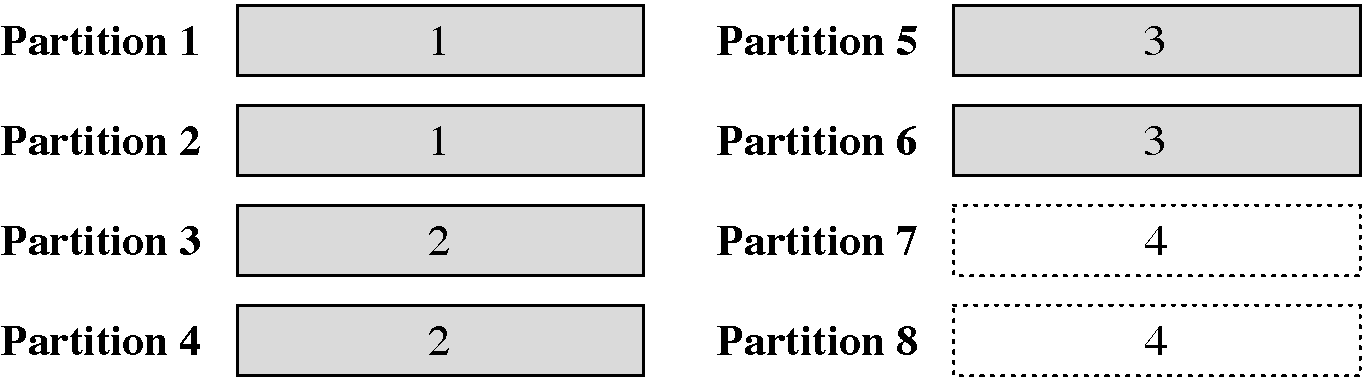
\includegraphics[width=\textwidth]{fault_tolerance/figures/disk_failure_before_recovery}
    \caption{\label{fig:disk_fail_before} The state of the job's intermediate
      partitions after the failure of disk 4. All intermediate partitions
      stored on disk 4 has been lost.}
  \end{subfigure}\hspace{0.05\textwidth}
  \begin{subfigure}[t]{\columnwidth}
    \centering
    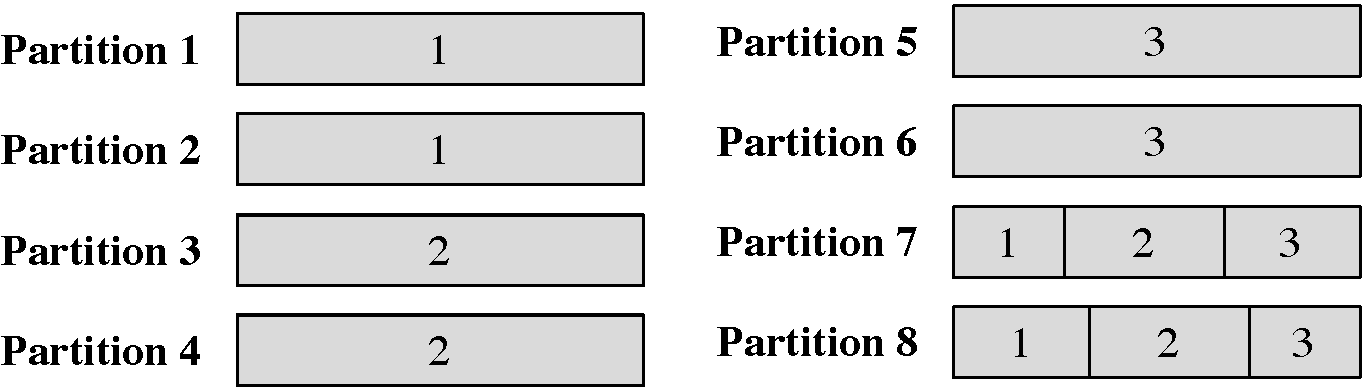
\includegraphics[width=\textwidth]{fault_tolerance/figures/disk_failure_after_recovery}
    \caption{\label{fig:disk_fail_after} The state of the job's intermediate
      partitions after recovery from the disk failure. Intermediate data for
      the partitions on disk 4 have spread across disks 1 through 3.}
  \end{subfigure}
  \caption{\label{fig:disk_fail} Illustrative example of disk failure and
    recovery in a two-node cluster with two intermediate disks per node and
    eight intermediate partitions. The rectangles
    representing each partition are labeled with the disk or disks on which
    data for that partition is stored.}
\end{figure}

Before we explore the technical details of the implementation, consider the
following illustrative example. Suppose that \themis is running on a two-node
cluster with two intermediate disks each, storing a total of eight intermediate
partitions for a particular job. In Figure~\ref{fig:disk_fail_before}, disk 4
in this cluster has failed during phase one, causing the loss of partitions 7
and 8. Figure~\ref{fig:disk_fail_after} shows the state of the intermediate
partitions at the end of phase one of the recovery job, when the data for
partitions 7 and 8 has been recovered.

Note that the recovered data for partitions 7 and 8 is spread across all the
remaining disks roughly evenly; this is highly desirable because it allows as
many disks as possible to participate in phase two of the recovery job. It
should also be noted that after the failure of disk 4 in phase one, phase two
can be run to completion on partitions 1 through 6 without waiting for the
recovery job to recover the other partitions.

\begin{figure}[t]
  \centering
  \begin{subfigure}[t]{\columnwidth}
    \centering
    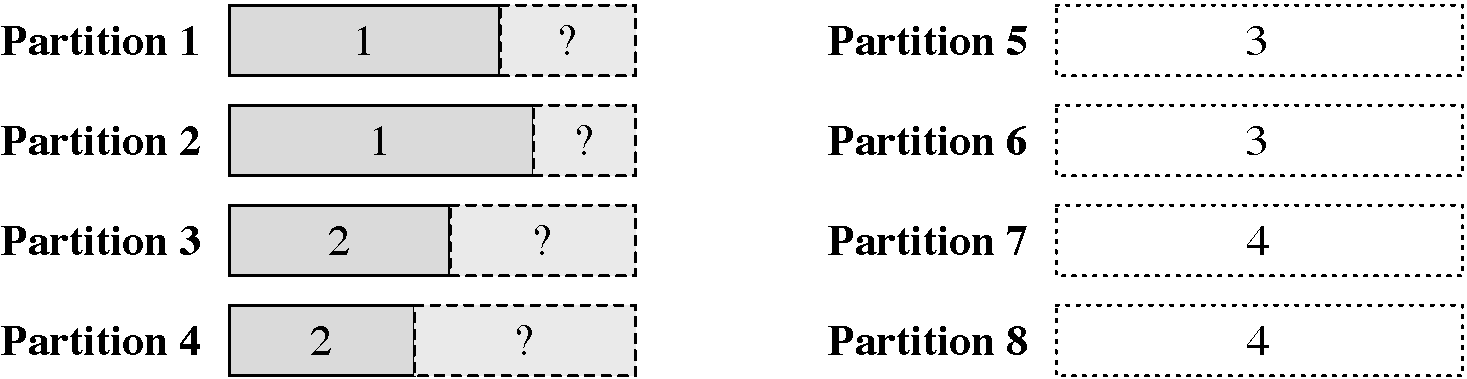
\includegraphics[width=\textwidth]{fault_tolerance/figures/node_failure_before_recovery}
    \caption{\label{fig:node_fail_before} The state of the job's intermediate
      partitions after the failure of node 2. All intermediate data for disks 3
      and 4 has been lost, and some data for the remaining partitions may not
      have been generated.}
  \end{subfigure}\hspace{0.05\textwidth}
  \begin{subfigure}[t]{\columnwidth}
    \centering
    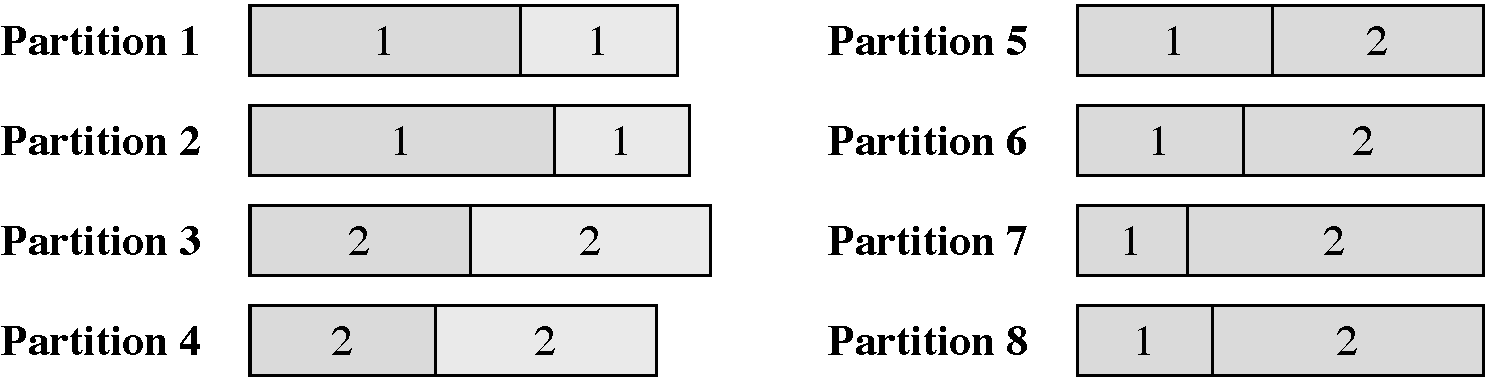
\includegraphics[width=\textwidth]{fault_tolerance/figures/node_failure_after_recovery}
    \caption{\label{fig:node_fail_after} The state of the job's intermediate
      partitions after recovery from the node failure. Intermediate data for
      the partitions on disks 3 and 4 have spread across disks 1 and 2, and
      data that should have been produced by node 2 has been added to node 1's
      partitions (although there may be duplicates).}
  \end{subfigure}
  \caption{\label{fig:node_fail} Illustrative example of node failure and
    recovery in a two-node cluster with two intermediate disks per node and
    eight intermediate partitions. A '?' indicates that it is unknown
    whether the data has been lost or not.}
\end{figure}

Figure~\ref{fig:node_fail_before} shows the same cluster after experiencing a
failure of an entire node. Not only have partitions 5 through 8 been lost, but
the remaining partitions are incomplete because the node did not finish
producing intermediate data for those partitions before it failed. Once phase
one of the recovery job has completed in Figure~\ref{fig:node_fail_after},
write recovery has spread the lost data from partitions 5 through 8 across
disks 1 and 2, while read recovery has ensured that every record that belongs
in partitions 1 through 4 has been written at least once.

\begin{table*}[t]
  \centering
  \caption{\label{table:failure_response} Table summarizing \themis' response
    to various kinds of failures at different points in the job.}
  \resizebox{\columnwidth}{!}{
  \begin{tabular}{|c|c|c|c|c|}
    \hline
    \textbf{Phase} & \textbf{Failure} & \textbf{Write Recovery} & \textbf{Read Recovery} & \textbf{Run Subsequent Phases?} \\
    \hline
    Zero (Sample) & Any & None & None & Yes \\
    One (Map + Shuffle) & Disk & Failed disk's partitions & None & Yes \\
    One (Map + Shuffle) & Node & All node's disks' partitions & Node's input files & No \\
    Two (Sort + Reduce) & Disk & Failed disk's partitions & None & Yes \\
    Two (Sort + Reduce) & Node & All node's disks' partitions & None & Yes \\
    \hline
  \end{tabular}
}
\end{table*}

In contrast to disk failure, phase two cannot be run after a node failure in
phase one because some intermediate partitions may not be complete.

If a disk or node fails in phase two, write recovery must be performed to
restore the intermediate data that was lost in the failure, but no read
recovery must be performed. Since phase zero is optional and does not produce
any output aside from a partition function, any failure during phase zero
simply requires re-executing it.

The responses to various kinds of failure in each of \themis' stages is
summarized in Table~\ref{table:failure_response}.

In the following sections, we will describe the mechanisms behind both write
and read recovery.

\subsubsection{Write Recovery}

To perform write recovery, the recovery job must re-map the failed job's input,
discarding any records that were not stored on the intermediate disks that
failed. To do this, the recovery job wraps its partition function in a
\emph{record filter}. This filter is applied to each record before it is passed
to the partition function. Abstractly, a record filter is a function that takes
a record as input and returns either ``accept'' or ``reject''. The filter
accepts a record if the record belongs to one of the partitions being
recovered, and rejects it otherwise.

In practice, \themis accomplishes record filtering in one of two ways. If the
failed job was using a user-defined partition function, the record filter
applies the failed job's partition function to the record. If the resulting
partition number is outside the range of partitions to be recovered, the filter
rejects the record.

If the original job is using a partition function generated by phase zero, the
record filter stores a set of boundary key ranges, one per contiguous range of
partitions being recovered. The complete list of boundary keys for each
partition is stored on distributed storage at the end of phase zero, and the
filter retrieves the appropriate boundary keys when it is constructed.

When an intermediate record is emitted by the \map function, the filter first
compares each intermediate record's key to the boundaries of each of its
ranges; if the record is within any of the filter's ranges, the filter
accepts the record.

In order to speed recovery by writing to as many disks in parallel as possible,
the intermediate data being recovered is spread across the cluster's remaining
intermediate disks. This is done by running phase zero during the recovery job
on a filtered sample of the input data, which generates a partition function
that spreads data in the filtered partition ranges evenly throughout the cluster.

At the end of phase one of the recovery job, any partitions that were
completely lost during a failure have been reconstituted and spread across the
cluster's remaining intermediate disks.

\subsubsection{Read Recovery}

As Table~\ref{table:failure_response} illustrates, read recovery is always
performed alongside write recovery. We take advantage of this by piggybacking
read recovery on write recovery.

In order to perform read recovery, we must first know the set of files that
were not completely processed by the failed node. \themis tracks which files
were completely mapped and received using a form of end-to-end
acknowledgments~\cite{endtoendargument}.  When a node is done reading a file in
phase one, it sends an EOF, or ``end-of-file'', annotation to every node in the
cluster indicating that the node will not receive any more data for the
file. Special care is taken to ensure that every intermediate record associated
with the file is transferred before this annotation. When a node receives an
EOF annotation, it adds the file's file ID to a list. At the end of phase one,
these lists are merged together to form a list of the nodes that received each
file. If every live node received an EOF annotation for a file, performing read
recovery on that file is not necessary. Each input file is checked for this
condition when constructing the input file list for a recovery job and files
are flagged for read recovery as appropriate.

Once phase one has completed, two sets of intermediate files will exist for the
failed job: the partially-complete set of files from the failed job and the set
of files generated as a result of read recovery. It is likely that some of the
records in these files are duplicates, and any duplicate records must be
removed to retain the \reduce function's correctness. To distinguish
intermediate records from one another, \themis tags each intermediate record
with \emph{source metadata} that uniquely identifies the record.

To uniquely identify intermediate records, we leverage the common assumption
that the \map function is deterministic and, as such, that applying the \map
function to an input record creates a totally-ordered sequence of intermediate
records. We identify an intermediate record by the position of its ``parent''
input record within the input dataset and its position in the totally-ordered
sequence of intermediate records. Specifically, we tag each record with a
64-bit file GUID, a 64-bit offset, and a 32-bit intermediate record ID. For the
purposes of evaluation, we store all 20 bytes of metadata even if the metadata
could potentially be compressed; note that for records with small offsets and
intermediate record IDs, these three pieces of metadata require far less than
20 bytes per record to store.

In phase two, intermediate partitions from the failed and recovery jobs with
the same intermediate partition number are concatenated together into an
in-memory buffer and sorted as a single intermediate partition. Before the
\reduce function is called on a set of intermediate records with a given key,
that set of records is secondarily sorted by its source metadata. The \reduce
function's record iterator then skips any records whose source metadata is the
same as that of the previous record.


\subsection{Multi-Tenancy in \themis}
\label{sec:multi-tenancy}

Each \themis node runs as a single process that assumes that it has exclusive
access to its intermediate disks and that it will not experience
memory pressure from other processes that results in swapping as long as it
does not exceed its configured memory limit. Its memory and disk management
subsystems (described in detail in~\cite{themis} and~\cite{tritonsort}) rely on
these assumptions and are the key enablers of \themis' I/O-efficiency and high
performance. Hence, running multiple \themis processes on a single node would
result in degraded performance since the processes would interfere with one
another.

\begin{figure}
  \centering
  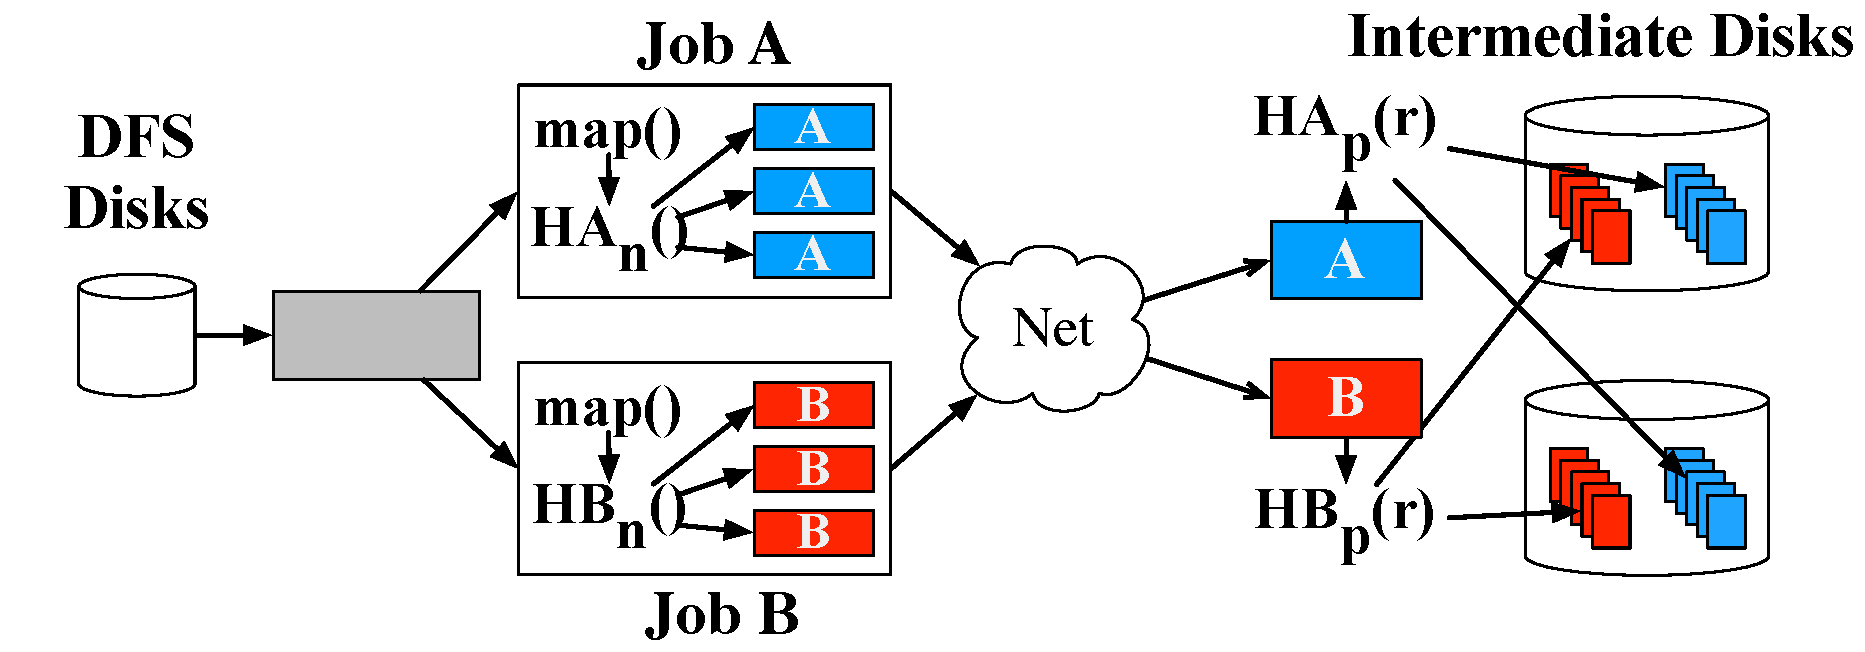
\includegraphics[width=\columnwidth]{fault_tolerance/figures/multi_tenancy}
  \caption{\label{fig:multi_tenancy} An overview of multi-tenancy in
\themis. Input records are mapped by both job A and job B's \map functions,
and intermediate records are routed based on each job's partition function independently.}
\end{figure}

To allow multiple jobs to run simultaneously in \themis with minimal
interference, we have modified \themis to support running multiple jobs
concurrently within a single process. To allow for this concurrent processing,
records read from disk are passed through each job's \map function one function
at a time, but intermediate records are transferred and written in
parallel. Buffers of intermediate records produced by a \map function are
tagged with the unique ID of that \map function's job before being sent to the
appropriate destination node. Once a buffer is received, this job ID is used to
determine to which set of intermediate partitions the buffer's records will be
written. This process is illustrated in Figure~\ref{fig:multi_tenancy}

A unique feature of our deployment prototype is that it does not co-schedule
\map and \reduce function computation. Instead, it organizes jobs into
\emph{batches}, and runs phases one and two for all jobs in a batch
simultaneously before processing the next batch. If phase zero needs to be run
to compute partition functions for any of these jobs, it is run on each job in
the batch individually before phase one starts.


\subsection{Job Dispatch}
\label{sec:control_plane}

The execution of batches of jobs is controlled by a \emph{cluster
  coordinator}. The cluster coordinator accepts descriptions of batches from
clients and coordinates their execution across the cluster's machines. Each
machine in the cluster runs a \emph{node coordinator} that is responsible for
running a \themis process on its machine and reporting an error if it crashes.

Messages are exchanged between the user, the cluster coordinator and the node
coordinators through the manipulation of message queues. Additionally, the
coordinators maintain metadata about both themselves and the jobs they run. In
our current implementation, the role of message queues and metadata store are
both filled by a Redis~\cite{redis} database. Redis was chosen primarily for
convenience; a scalable key-value store like Hyperdex~\cite{hyperdex} or
Cassandra~\cite{cassandra} and message queue like Kafka~\cite{kafka} or
Kestrel~\cite{kestrel} could be substituted.

To run a batch, the user pushes a description of the jobs in the batch to the
cluster coordinator's job queue. Upon dequeuing a batch, the cluster
coordinator assigns a unique job ID to each job in the batch. It then determines
the set of input files that each job will process, and divvies those files out
among nodes. We describe this process in more detail in
Section~\ref{sec:input_file_gathering}.


\subsection{Input Files and Distributed Storage}
\label{sec:input_file_gathering}

\begin{figure}
  \centering
  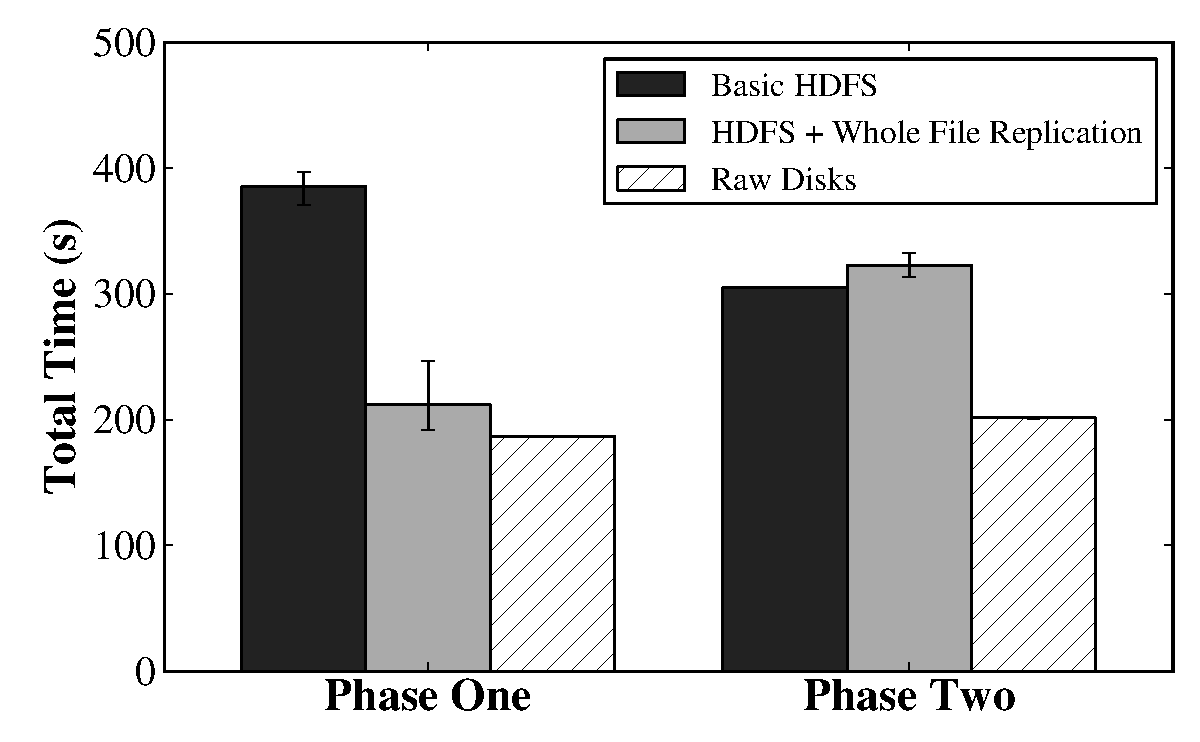
\includegraphics[width=\columnwidth]{fault_tolerance/graphs/hdfs_no_proxy_penalty}
  \caption{\label{fig:hdfs_no_proxy_penalty} Comparing the performance of
    unmodified HDFS, HDFS with whole file replication for the primary replica,
    and reading and writing from raw disks.}
\end{figure}

The specification of each \themis job includes an input directory; all files in
the input directory are processed. \themis can read input files from raw disks
or from HDFS~\cite{hdfs} using the WebHDFS REST API. We use HDFS exclusively in
this work.

Each file is uniquely identified by its URL, which is of the form\\
\texttt{<protocol>://<host>:<port>/<path from root>}. Each file is also given a
file ID that must be unique within the job. In our implementation, a
file's ID is the upper 64 bits of the MD5 hash of its URL.

Our main concern when moving from raw disks to distributed storage was
maximizing the amount of bandwidth we could achieve from the storage system.
In order to achieve sufficient bandwidth, we found that we needed to change the
way HDFS allocates blocks for files. In particular, we modified HDFS so that it
performs \emph{whole-file replication} of the file's primary replica by placing
every block on a specific disk in the cluster based on the file's name. For
example, a file named \texttt{/1.2.3.4/3/<path>} would be stored on the third
DFS disk on node \texttt{1.2.3.4}. To allow \themis to remain oblivious to this
scheme, we implemented a proxy that performs a basic round-robin allocation of
primary file replicas to cluster disks and transparently maps between regular
and placement-aware paths. The proxy only interposes itself in communication
between \themis and HDFS when a file is first opened, and imposes no additional
overhead thereafter.

Figure~\ref{fig:hdfs_no_proxy_penalty} compares the performance of an 800GB, 8
node sort with and without these modifications; as a reminder, phase one of
\themis reads sequentially from HDFS, while phase two writes sequentially to
it. The substantial performance improvement for reads is the result of the
elimination of read contention on each node's DFS disks when many files are
being read simultaneously. However, the increased rigidity of block allocation
imposed by the proxy makes the performance of writes slightly worse than
unmodified HDFS.

We found that HDFS' block placement APIs were not sufficient for providing
whole-file replication for all of a file's replicas. Hence, blocks for all
other replicas are allocated according to HDFS' default policy, and access to
non-primary replicas occurs at the speed of unmodified HDFS. The cluster
coordinator will assign files to nodes that contain their primary replica
whenever possible.


\subsection{Responding to Failures}
\label{sec:fault_response}

As node coordinators run, they refresh a keep-alive key in Redis every few
seconds; if a node fails to refresh its keep-alive key, the cluster coordinator
presumes that the node has failed. A node notifies the cluster coordinator
directly if it finds that it can no longer write to one of its intermediate
disks.

\themis attempts to insulate the rest of the cluster from a failure whenever
one occurs so that the healthy portion of the cluster can complete as much work
as possible. To avoid the attendant complexity and fragility of coordinating
failure notification across nodes, \themis simply discards any data meant for a
failed portion of the cluster. When a node fails, all existing TCP sockets to
that node will break. Nodes respond to broken sockets by discarding all data
meant for that socket for the remainder of the batch. Similarly, when a disk
fails, all data that would have been written to the failed disk for the rest of
the batch is discarded. Subsequent batches will not use failed disks or nodes
until an operator has explicitly marked them as having recovered.

Currently, the user is responsible for issuing a recovery job to recover a
failed job. Scheduling recovery jobs to maximize the likelihood of scan sharing
is beyond the scope of this work; we examine some related efforts relevant to
this problem in Chapter~\ref{chapter:related_work}.

